\chapter{Characterization of a Gravitational Wave Detector}

As discussed in section \ref{sec:ihope_far}, the CBC group measures the
significance of candidate events by comparing the combined new SNR
against the background distribution.  The background is obtained by
sliding the triggers from each IFO against each other by more than the
light travel time between them.  In the limit of at most one real
gravitational wave in each analysis segment this ensures that the
background is composed entirely of triggers resulting from non-
gravitational-wave sources.

Ideally, the instrumental noise would be Gaussian and the only source
of extraneous triggers would be random fluctuations.  In reality
environmental couplings to the instrument, such as electrical and
seismic, as well as glitches within the instrument will also produce
triggers.

It is in the interest of the collaboration to remove as many of these
triggers as possible so that any real events will stand out 
well above the background.  This removal must be done in
an automated way in advance of looking at the results from the
analysis.  LIGO would be justly criticized if the background were
to be adjusted after the analysis in order to make a marginal candidate
appear more significant.

There is therefore a need for a process of detector characterization
(henceforth ``detchar''), a way to remove times from the analysis that
are more likely to produce triggers from noise than from a real event.
One of the most significant features of the S6 run is that the people
working on detchar were in close contact with the people commissioning
the instrument.  This meant that, in addition to cleaning the search,
information about problematic behavior in the instrument could be used
to fix the problems at the source, in turn allowing more time to be
analyzed and the prospects for making a detection to improve.

Detchar was a major undertaking, much more information can be found in
(Smith and Lundgren in progress).  Here we focus on the \emph{segment
database}, a key piece of infrastructure, and \emph{daily ihope}, a
modification of the CBC search used for detchar.


\section{The Segment Database}

\subsection{Data Quality Flags}

The state of the instrument at any time is summarized by a set of
\emph{flags}.  Flags are identified by a triple of (ifo id, flag name,
version number), where \emph{ifo id} identifies the instrument,
\emph{flag name} is a unique identifier, and \emph{version number} is
an integer starting from 1.  The version number allows information to
be updated without losing information that may be needed to
reconstruct the results of earlier searches.  The full set of flags is
stored in a database designed at Syracuse and hosted at Caltech.

Flags are stored as a set of \emph{segments}, half-open intervals
aligned on GPS integer second boundaries.  Each flag triple has an
associated set of segments indicating the times during which it is
\emph{defined}.  Such triples also have a set of segments indicating
times during which they are \emph{active}.  The set of active segments
must be a subset of defined segments.  Times during which a flag is
defined and not active are considered \emph{inactive}.

Flags may be entered manually through a web interface.  This can be
used to indicate nonstandard operating conditions, such as heavy
equipment being operated on site.  However, most flags are generated
automatically.

The first line of defense against noise triggers is on-site as the
instrument is running.  At all such times the control room is staffed
by an operator who is an expert in running the instrument employed by
LIGO labs, and a science monitor (``SciMon'') who is a member of the
LIGO Scientific Collaboration.  The two jointly decide when to enable
\emph{science mode}, which marks the data as suitable for analysis.
This declaration is not specific to the CBC group, but extends to all
searches in the collaboration.  Science time is indicated by the flag
\texttt{DMT\_SCIENCE}.

In addition to the readout channel (\texttt{DARM\_ERR}, section
\ref{sec:inst_readout} many other data channels are recorded, falling
into two broad categories.  Physical environmental monitor (``PEM'')
channels record information about the environment such as seismic
activity at the base and end stations, microphones and magnetometers
placed throughout the site, etc.  Instrumental (``INST'') channels
record data from numerous subsystems such as servos for each mirror
and the output of photodiodes at points throughout the light path.
Software running at the sites called the data monitoring tool
(``DMT'') creates data quality flags based on these channels.  For
example, when a channel's value or standard deviation over time
exceeds a given threshold.  The DMT is also responsible for recording
the state of the science mode flag.  Other flags are set by programs
that run analyses on these auxiliary channels, for examples see
(\checkme{UPV refs}).


\subsection{The Veto Definer}

Problems in the data may have differing levels of severity, and
consequently we define several \emph{veto categories} to characterize
them.  The categories used by daily ihope differ slightly from those
used by the full analysis.

Category 1 vetoes indicates time that should not have been marked as
science mode.  Typically attempting to analyze this time will
adversely affect the entire 2048-second analysis chunk, for example by
biasing the PSD (section \ref{sec:ihope_psd}).  Note that it is
possible to correct science time by creating a new version of the
\texttt{DMT\_SCIENCE} flag with an incremental version number.
However, doing so is a more complicated process than creating a veto
flag, and removing time by denoting it CAT1 carries additional
information about the reason for the veto.  Note that category 1
vetoes are undesirable, as they may remove time outside the range of
the problem.  For example, a 4080-second span of science-mode data
with a one-second CAT1 veto at 2040 seconds will be completely
unanalyzable by the CBC group, as excising the bad data will leave no
contiguous 2048-second block.

Category 2 vetoes indicates time during which there was a problem,
instrumental or environmental, with well-understood coupling into
\texttt{DARM\_ERR}.  Such time can be analyzed without problem, but
triggers from such time will be discarded. 

Category 3 vetoes remove hardware injections (section
\ref{sec:ihope_hardware_injections}).  In the full analysis hardware
injectiob vetos do not have a category number and is denoted
``hardware injections removed.''

Category 4 is for time that appears to be ill-behaved according to 
data quality studies, but where there is no clearly-understood 
cause.  In the full analysis this is denoted category 3.

Finally, a map is needed between data quality flags and veto
categories.  This is achieved through the use of a search-specific
\emph{veto definer file} which associates a flag with a veto level.
Intervals within the range during which that version of the flag are
active will be marked with the corresponding veto level.  The
\texttt{ligolw\_segments\_from\_cats} program (see below) merges the
information in this file with the set of active flag segments to produce
\emph{veto segments} at each veto level.  Analysis is performed on
times marked as science with no CAT1 vetoes.  Triggers from times
marked as CAT2, CAT3 and CAT4 are discarded from both foreground and
background.

Sometimes the threshold on a DQ flag is such that the data is
unsuitable for analysis close to, but outside, the range of the flag.
The veto definer file therefore allows for \emph{padding}, offsets 
which effectively extend the flags.


\subsection{Technical details}

The flag segments are stored in a high-performance relational
database, exposed as a web service which provides secure access to all
members of the collaboration.  Several utilities to interact with the
segment database were written, many of which could run in many modes.
The names of all these utilities start with ligolw, short for ``LIGO
lightweight,'' an XML-based format used throughout the collaboration
in which the output was generated.

Except where noted all programs accept a common subset of arguments
\begin{itemize}
\item \texttt{--gps-start-time} and \texttt{--gps-end-time}: Integer
GPS times specifying the time range over which to run.
\item \texttt{--include-segments}: Takes a comma-separated list of
segment specifiers of the form ifo:flag\_name:version or
ifo:flag\_name and restricts the query to matching flags.  In the
latter case, report on the latest version of the flag defined at each
time within the time range.
\item \texttt{--exclude-segments}: Takes a comma-separated list of
segment specifiers in the same format as \texttt{--include-segments}.
Runs a second query on the excluded segments and returns the set of
segments in included segments - (included segments $\cap$ excluded
segments).
\item \texttt{--database}, \texttt{--segment-url},
\texttt{--dmt-files}: Specifies the data source (segment database or
XML files with segment information).
\end{itemize}


The programs used during S6 were:

\textbf{ligolw\_dq\_query}.  This program reports on the state of
flags at one or more GPS times given on the command line.  This
program does not support \\
\texttt{--gps-start-time} or \texttt{--gps-end-time}.   The available modes are

\begin{itemize}
\item \texttt{--report}:  Returns the active/inactive status of all DQ flags at the
given times.  For active flags reports the start and end times of the
segment within which the given time is contained.  For inactive flags
reports the end time of the nearest preceding segment and the start
time of the nearest subsequent segment.  This mode is used in the
daily ihope ``loudest glitches'' page, see below.
\item \texttt{--defined}: Returns a list of flags defined at the
given times.
\item \texttt{--active}: Returns a list of the flags that were active
at the given times.
\item \texttt{--start-pad}, \texttt{--end-pad}: Extends the
\texttt{--defined} and \texttt{--active} modes to report on the status
of flags within a small range of time.
\end{itemize}


\textbf{ligolw\_segment\_query}.  This program reports on the state of a
set of flags over a span of times.  The available modes are

\begin{itemize}
\item \texttt{--show-types}: Reports the sets of flags that exist over
the time span.
\item \texttt{--query-types}: Reports the segments during which the
flags were defined.
\item \texttt{--query-segments}: Reports the segments during which the
flags were active.
\end{itemize}

Every CBC analysis begins by determining the science mode times with a
call of the form

\vspace*{5mm}
\texttt{ligolw\_segment\_query} \\
\hspace*{0.5in}\texttt{--query-segments --include-segments H1:DMT-SCIENCE:3 ...}
\vspace*{5mm}

\textbf{ligolw\_segments\_from\_cats}.  Given a veto definer file,
report on segments to be vetoed. 

\textbf{ligolw\_dq\_active\_cats}.  Given a veto definer file and GPS
time, report on the active/inactive status and veto category for all
flags defined at the time.

\textbf{ligolw\_segment\_insert}.  Adds new segments to the database,
enforcing various policy decisions:
\begin{itemize}
\item New segments for an existing flag/version number pair must not overlap 
with existing segments.  To update information a new version number must be used.
\item New version numbers must be one greater than the largest
existing version number.
\item New segments must not extend into the future, past the GPS time
at which the program is run.
\end{itemize}


% https://www.lsc-group.phys.uwm.edu/daswg/wiki/content_of_segment_publication_and_discovery


\section{Daily ihope}


As discussed in (search chapter) the CBC group uses the \emph{ihope}
pipeline to search for gravitational waves produced by the inspiral of
binary systems consisting of neutron stars and/or black holes.  During
LIGO's 6th science run (July 7, 2009 - October 20, 2010) which
overlapped Virgo's second (July 7, 2009 - January 11, 2010), and third
(August 11, 2010 - October 20, 2010) science runs, the goal of the
group was to run the full analysis every two weeks with latencies as
small as possible.  The daily ihope runs were conceived of as a way to
characterize the detector in order to look for potential problems in
advance of the full search, particularly problems specific to the CBC
search.

It is important to stress that daily ihope was not itself a
gravitational wave search, it was a tool to help determine whether the
data in each instrument was suitable to analyze.  This goal determined
the specifics of the daily runs, but more significantly it leaves the
full search unbiased.

Recall that ihope is a templated, matched-filter search.  For the
low-mass search, which was the focus of the daily runs, the templates
are restricted, stationary-phase frequency-domain waveforms with phase
evolution taken to 3.5 PN order.  The templates are laid out in a bank
with 97\% overlap between nearest neighbors, and the mass range is
from 2 $\msun - 25 \msun$.  A $\chisq$ discriminator is constructed to
better separate signals from glitches (eqn \ref{eq:analysis_chisq} ,
and the information from this discriminator is used along with the SNR
to construct the new SNR detection statistic (eqn
\ref{eq:analysis_newsnr}).

By construction a great deal of the information provided by
the full bank search is redundant.  Further, the evaluation of each
additional template and the initial layout of the bank incurs
significant computational overhead.  Therefore a number of
simplifications were applied to the daily ihope bank.

First, a static bank was used for each IFO, based on the layout at a
quiet time in each instrument.  Second, the number of templates was
reduced.  Lower-mass systems have more cycles in the sensitive LIGO
band, there is therefore ample information to distinguish between
waveforms with close parameters.  Conversely, this means that the
low-mass end of the bank is very dense (in the sense of number of
templates per unit square in parameter space, they are still
equidistant in the sense of eq. \ref{eq:analysis_match_filter}).  Such
fine resolution is not needed when looking for glitches, therefore the
minimal match between templates in the region below a chirp mass
($\mathcal{M} = M \eta^{3/5}$) of 3.46 $M_\odot$ was set to 0.5.  At
higher masses, up to a total mass of $25 M_\odot$, the minimal match
was set to 0.95.  In addition to ensuring coverage in a mass region
which is naturally sparser this ensures that short glitches,
characteristic of many glitch mechanisms, were flagged with large
SNRs.  The resulting hybrid bank for the Hanford detector is shown in
figure \ref{f:daily_ihope_bank}.

\begin{figure}
  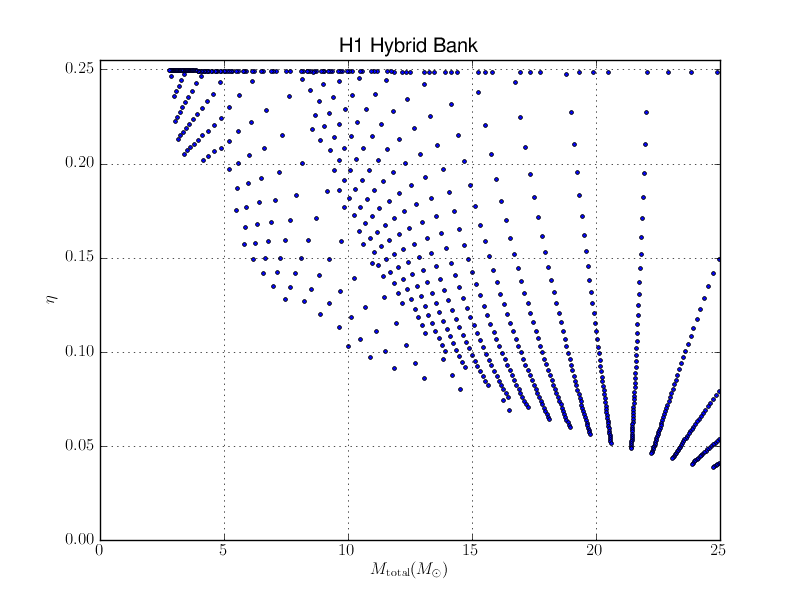
\includegraphics[width=\linewidth]{figures/detchar/hybrid_bank.png}
  \caption{The hybrid template bank used by daily ihope for the
Hanford detector.  The cut is made at constant chirp mass, which is
a curve in the total mass, $\eta$ plane.}
  \label{f:daily_ihope_bank}
\end{figure}%

Daily ihope processing ran at 03:00 GMT and examined data spanning the
24 hours ending at 00:00 GMT.  Unlike full ihope, the analysis was
done on all science time, including that which would be vetoed at CAT
1 by the full analysis.  This was done so that we could see the effect
of the CAT 1 vetoes.  It is plausible, for example, that some such
vetoes would be too aggressive and we could decide based on the daily
results to include such times back into the analysis.  For consistency
science time was denoted CAT 0.  In addition CAT 3 vetoes to remove
hardware injections were not applied, so that we could see how many
injections would be lost by CAT 4 vetoes.  The daily pages therefore
displayed results for categories 0, 1, 2, and 4.

For each 2048-second chunk of contiguous data, at each IFO, the data
was run through each template in the bank and triggers selected as
described in section \ref{sec:analysis_trigger_selection}. For each
trigger $\chisq$ and new SNR were calculated and recorded.  Clustering
was then done in order to focus attention on glitches that were most
likely to cause problems in the full search.  Two sets of clustered
triggers were recorded using windows of 30 milliseconds and 16
seconds.  For each set the trigger with the largest value of new SNR
across all templates within the window length was recorded.

The triggers were also filtered.  A version of the veto definer file
designated as ``online'' was maintained and used by daily ihope to
identify times with veto categories.  These vetoed times were then
removed from the original and clustered files.  
% The pipeline is summarized in figure (xx).
The result is, for each 2048-second block in each ifo, 3 cluster
levels times 4 veto levels = 12 sets of triggers.

%do analysis
%record science triggers
%cluster 30 ms     determine cat 1
%cluster 16 sec    determine cat 1 + cat 2
%                  ...

%filter and record

Several plots and reports were generated for each combination
of veto level and cluster level.

\subsection{Analysis time and veto usage}

This report shows the total time analyzed, the vetoes applied beyond
those applied at the previous level, the \emph{efficiency} (percentage of
triggers removed) and \emph{deadtime} (percentage of time removed) by
each veto.  In addition the ratio of efficiency over deadtime is
reported as a measure of quality of the veto.  A random veto would
result in an efficiency-over-deadtime of approximately 1, a
finely-tuned veto that removes short, loud events that ring off the
entire template bank would have a much higher ratio.

This allowed analysts tuning the veto definer files to get an ongoing
measure of how well vetoes were working.

\begin{figure}
  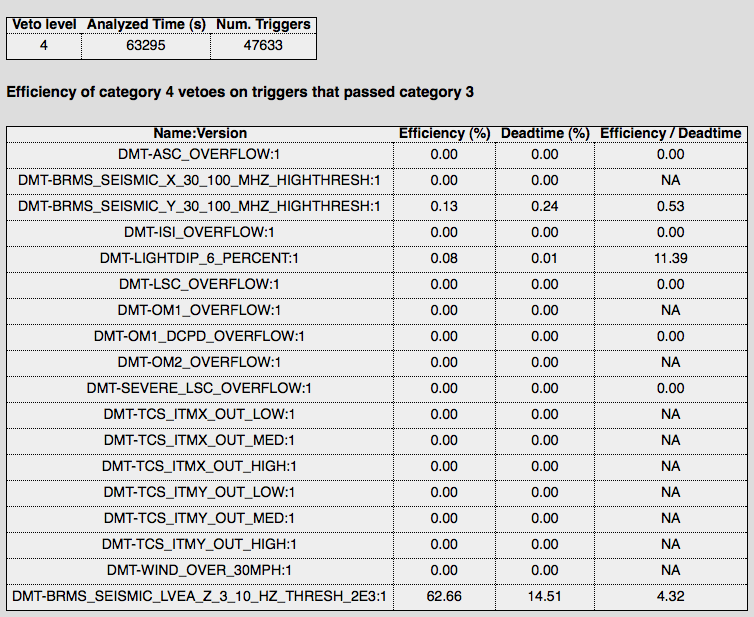
\includegraphics[width=\linewidth]{figures/detchar/vetousage.png}
  \caption{Sample veto usage report from Aug 19, 2010.  See text for
explanation.  Note that 62.66\% of all triggers were contained in
14.51\% of time, and the DMT flagged this time with elevated
seismic activity from 3-10 Hz at the LVEA}
  \label{f:daily_ihope_vetousage}
\end{figure}%

\subsection{Loudest Triggers}

This report was only run for 16-second-clustered triggers.  Loud
glitches tend to produce families of triggers,  without clustering the
loudest triggers from each day would likely result from one underlying
event.  This report considers two classes of triggers; those where no
data quality flag was active and those where at least one flag was
active.  For the five triggers with highest new SNR in each category a
summary was presented along with a link to an \emph{omega scan}.  The
omega pipeline is described in (\checkme{omega refs}).  Omega scans
are a kind of time-frequency plot.  They are especially useful as they
may be run on all auxiliary channels recorded by the instruments and
therefore provide a visual aid to detecting coupling between auxiliary
channels and the gravitational wave readout channel.

These can be used to suggest mechanisms behind glitches, especially
those that were not already marked by a DQ flag.  In addition, over
time repeated shapes in the omega scan can pinpoint underlying
problems in the instruments that need to be addressed.

(note that the dog showed up in this list at both H1 L1)

\begin{figure}
  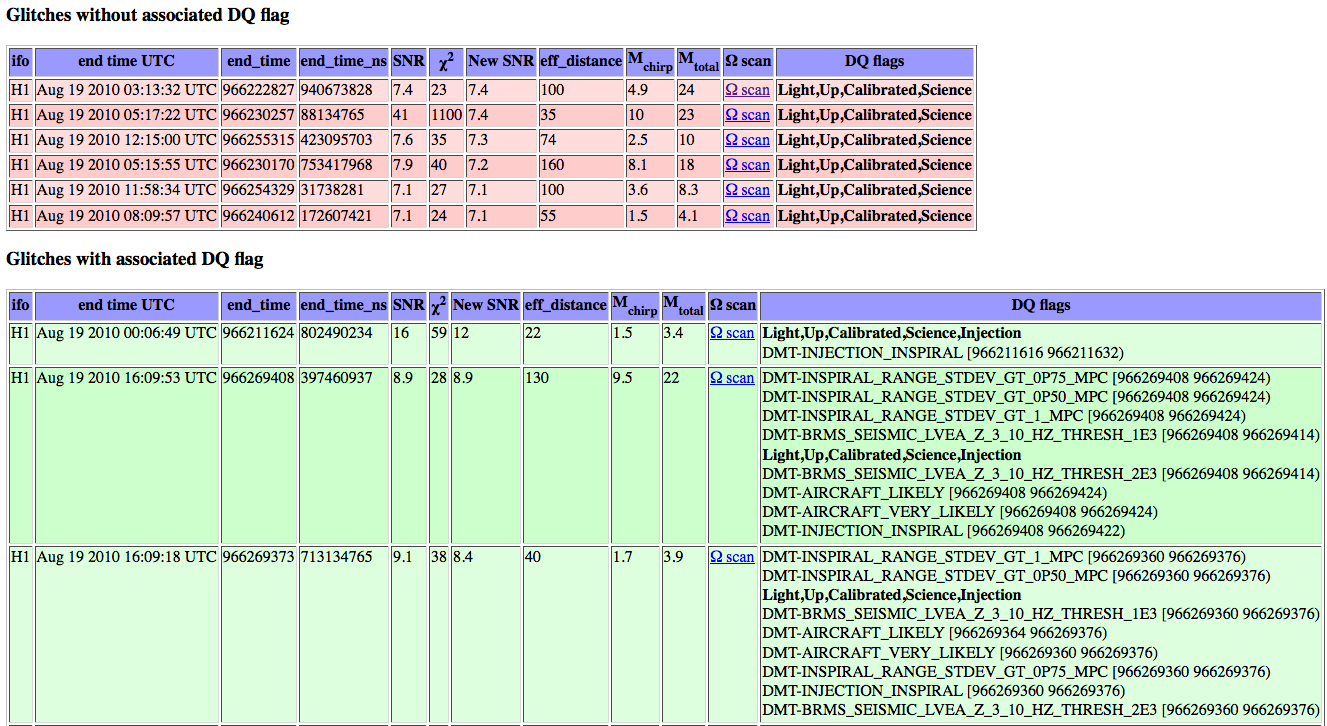
\includegraphics[width=\linewidth]{figures/detchar/loudest.png}
  \caption{Sample loudest trigger report from Aug 19, 2010.  See text for
explanation.  Note the rightmost column is populated by the
\texttt{ligolw\_dq\_query} program in the \texttt{--report} mode. }
  \label{f:daily_ihope_loudest}
\end{figure}%



\begin{figure}
  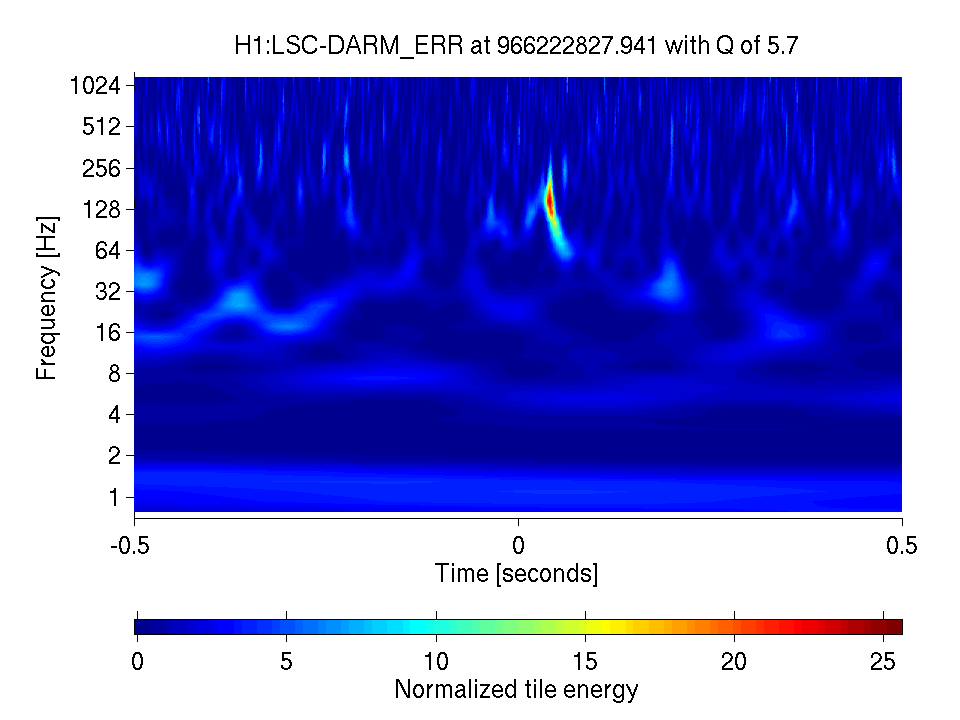
\includegraphics[width=0.5\linewidth]{figures/detchar/966222827_940673828_H1_LSC-DARM_ERR_1_00_spectrogram_whitened.png}
  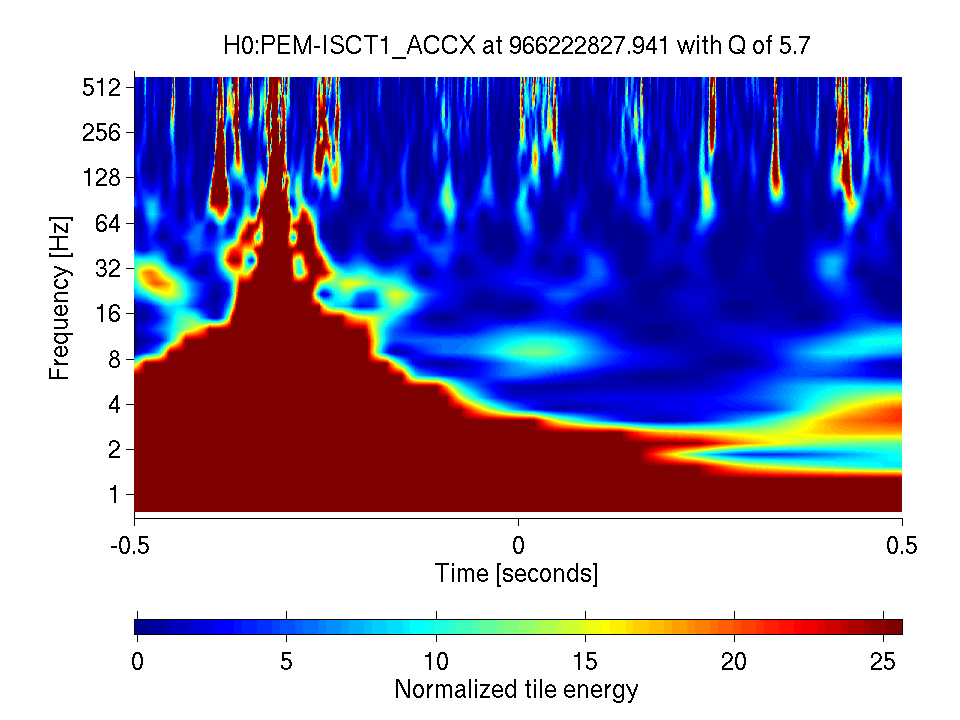
\includegraphics[width=0.5\linewidth]{figures/detchar/966222827_940673828_H0_PEM-ISCT1_ACCX_1_00_spectrogram_whitened.png}
  \caption{Omega scans from the loudest H1 trigger in figure
\ref{f:daily_ihope_loudest}.  Note the trigger closely follows a loud
event in one of the accelerometers on an instrument table.}
  \label{f:daily_ihope_loudest_omega}
\end{figure}%


\subsection{HW Injections}

This report was generated by code written by John Veitch  at Cardiff
University.  It compared the list of injections, published as an XML
file available from a web site, with the list of analysis times and
triggers.  The results were plotted to indicate whether each injection
was found, missed, or not analyzed.

\subsection{SNR Histograms}

These plots show the number of triggers as a function of SNR and new
SNR.  As noted in section \ref{sec:ihope_match_filter}, in Gaussian
noise the number of triggers should be proportional to
$\exp(-\rho^2/2)$.  These plots therefore show the degree of
``non-Gausianity'' in the data.  A common use for these plots was to
flip between veto levels to get a sense of how well the cumulative
vetoes were cleaning the data, as shown in figure
\ref{f:daily_ihope_gaussianity}.


\begin{figure}
  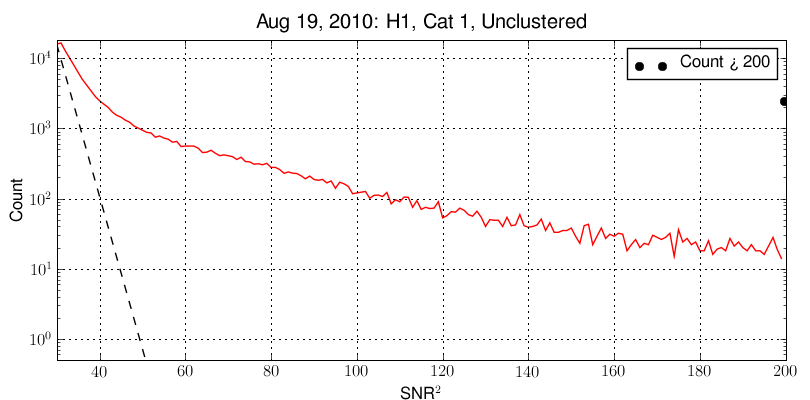
\includegraphics[width=0.5\linewidth]{figures/detchar/H1_1_UNCLUSTERED_snr_hist.png}
  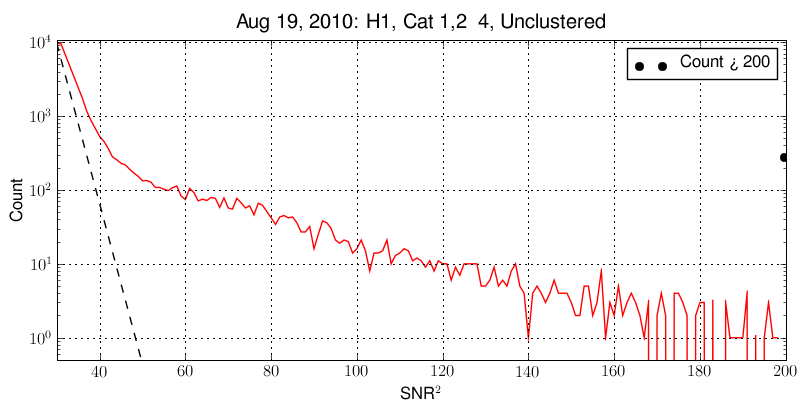
\includegraphics[width=0.5\linewidth]{figures/detchar/H1_4_UNCLUSTERED_snr_hist.png}
  \caption{Trigger histograms for H1.  The dashed line shows the
expected values in Gaussian noise.  The dot indicates the cumulative
number of triggers with new SNR greater than 200.  Note that at veto
category 4 (right) the histogram is closer to the expected line than
it is at category 1 (left).  This indicates the degree to which data
quality has removed non-Guassian noise.}
  \label{f:daily_ihope_gaussianity}
\end{figure}%


\subsection{Glitchgram}

The ``glitchgram'' was an ``at-a-glance'' summary of the day, showing
every trigger color-coded by SNR.  This highlighted times of loud
triggers as well as dense regions indicating ``grumbly'' times.  A
sample is shown in figure \ref{f:daily_ihope_glitchgram}.

\begin{figure}
  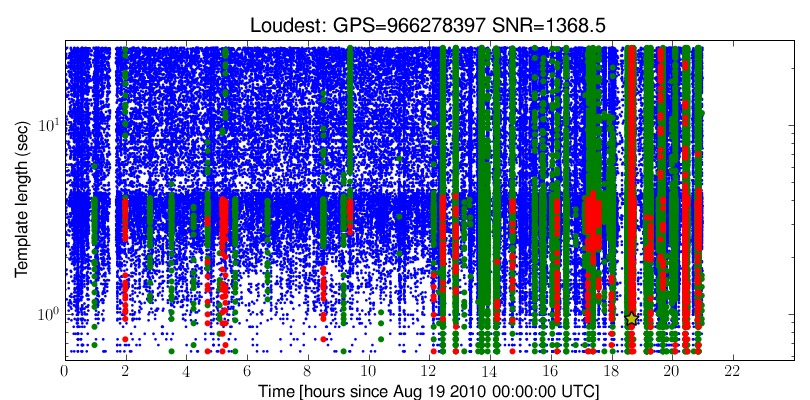
\includegraphics[width=\linewidth]{figures/detchar/H1_1_UNCLUSTERED_glitchgram.png}
  \caption{The Aug 19th daily ihope ``glitchgram.''  Blue dots have
new snr values below 8, green have values between 8 and 16,
and red have values above 16.  Template length was chosen as the Y
axis in order to capture a feature of the templates that is not
specific to gravitational wave signals, such as chirp mass.
Note the break at 4.3 seconds, corresponding to the
chirp mass at which the bank switches from an overlap of 0.95 to 0.5.
Comparing to figures 3 and 4 shows the same 
excess of triggers after 12:00.  No data is analyzed after 21:00
because ihope requires at least 2048 contiguous seconds to estimate
the PSD and all data after this time was in smaller segments.}
  \label{f:daily_ihope_glitchgram}
\end{figure}%


\subsection{Rate vs. Time and SNR vs. Time}

These plots complimented the glitchgram by breaking the triggers up
differently.  The rate plot showed average number of triggers over
1-minute intervals.  The SNR plot showed the SNR of every trigger as a
function of time.  These tend to be correlated, as loud glitches ring
off the entire bank and produce large numbers of triggers.

The plots were accompanied by tables showing the times where the
rate of triggers exceeded 500 Hz for more than one second, and
exceeded 200 Hz for more than 10 seconds.

\begin{figure}
  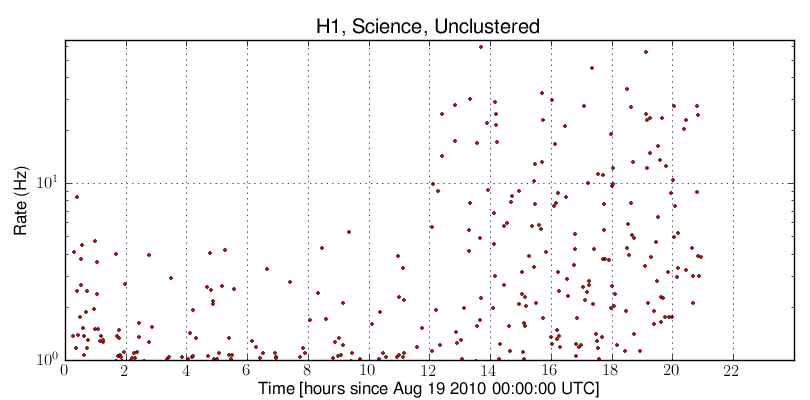
\includegraphics[width=\linewidth]{figures/detchar/H1_0_UNCLUSTERED_rate_vs_time.png}
  \caption{Daily ihope rate plot, showing rate in Hz (averaged over
1-minute intervals) as a function of time.  Note that the rates
increase after 12:00.  This was due to increased seismic noise.}
  \label{f:daily_ihope_rate_v_time}
\end{figure}%

\begin{figure}
  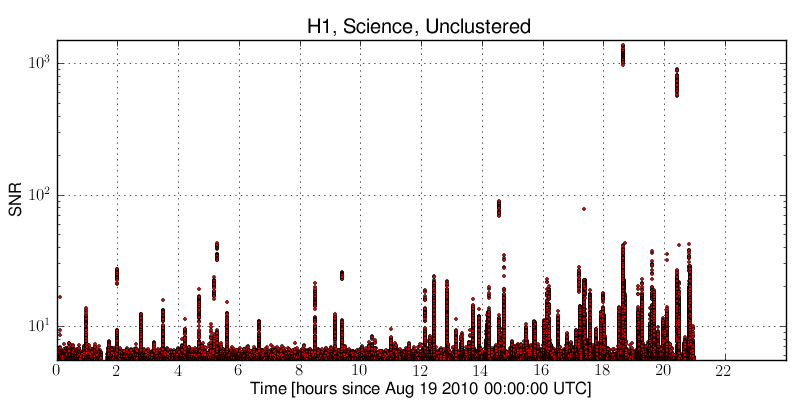
\includegraphics[width=\linewidth]{figures/detchar/H1_0_UNCLUSTERED_snr_vs_time.png}
  \caption{Daily ihope SNR plot as a function of time.  The density of
triggers increases somewhat after 12:00 and there are more loud
outliers.  However the change in behavior is better seen in 
figure \ref{f:daily_ihope_rate_v_time}.}
  \label{f:daily_ihope_snr_v_time}
\end{figure}%
% \subsection{Breakdown by template}

\subsection{Chi-square test}

These plots showed all triggers in with SNR values on the $x$-axis and
$\chisq / (2p-2)$ (the reduced $\chisq$) on the $y$-axis as a way to
visualize the glitchiness of the data.  These plots are most useful
when compared to a reference plot generated from a day of simulated
Gaussian noise, shown in figure \ref{f:gaussian_snr_chisq}, and
comparing the plots at different veto levels, shown in figure
\ref{f:daily_ihope_snr_chisq}.

\newpage
\begin{figure}
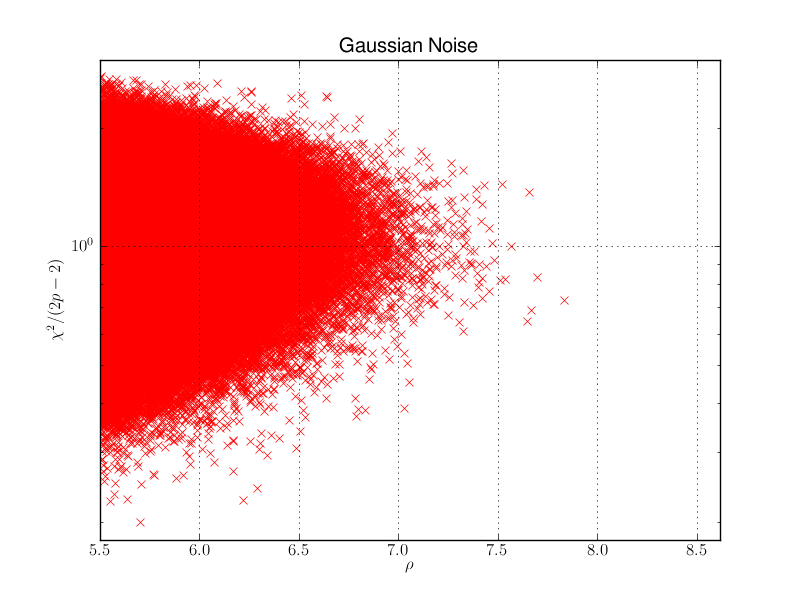
\includegraphics[width=0.85\linewidth]{figures/detchar/GAUSSIAN_0_UNCLUSTERED_chisq.png}
\caption{The SNR/reduced $\chisq$ plane for a reference day of
Gaussian noise.  This is the product of a $\chisq$ distribution on the
$y$ axis and a Gaussian distribution on the $x$ axis.}
\label{f:gaussian_snr_chisq} \end{figure}%

\begin{figure}
  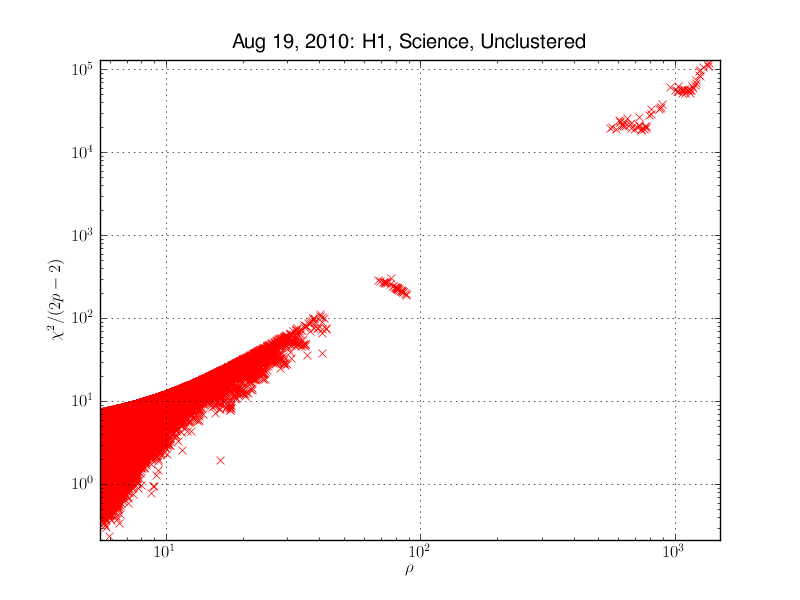
\includegraphics[width=0.5\linewidth]{figures/detchar/H1_0_UNCLUSTERED_chisq.png}
  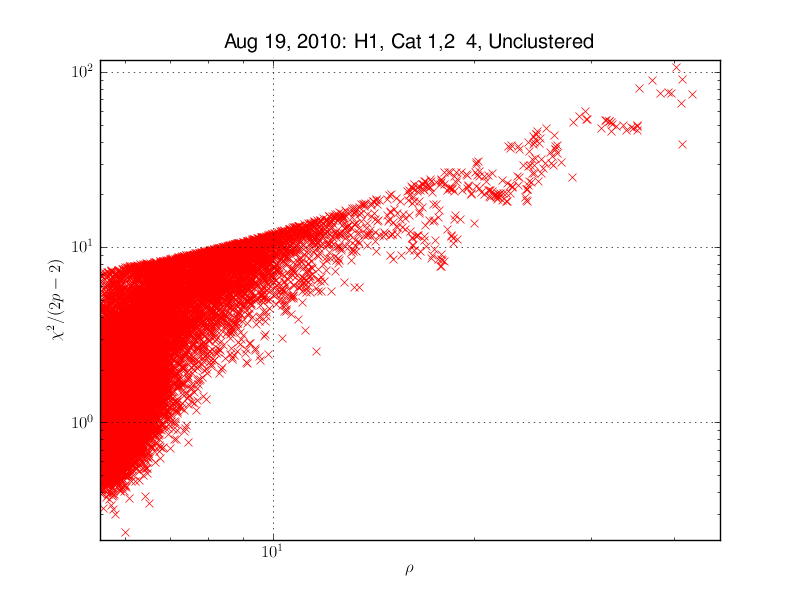
\includegraphics[width=0.5\linewidth]{figures/detchar/H1_4_UNCLUSTERED_chisq.png}
  \caption{SNR/reduced $\chisq$ plots of H1 data.  The expected shape
of figure \ref{f:gaussian_snr_chisq} is discernible, but there are
long tails of non-Gaussian glitches.  The sharp cutoffs arise 
from thresholds within the inspiral code, see section
\ref{sec:analysis_trigger_selection}.  There is a further
population extending to the upper right at category 0 (left) that is
removed by vetoes in category 4 (right).}
  \label{f:daily_ihope_snr_chisq}
\end{figure}%
\newpage
\section{Applications of daily ihope}

In addition to the hardware injections discussed in section
\ref{sec:ihope_hardware_injections} it was known at the start of S6
that there would be any from zero to ``a few'' unannounced, blind
hardware injections performed in order to provide an unbiased test of
the search pipelines.  One such injection was performed on  Sep 16
2010 at 06:42 UTC, and showed up in multiple searches as a strong
gravitational wave candidate.  This candidate was followed up to the
point of writing a detection paper and submitting it to the
collaboration for publication approval.  Once approval had been
granted the fact that it had been an injection was revealed.  For more
details on the event and how it was followed up, see (the S6 low mass
paper).

Although daily ihope was not a search, the injection showed up on the
page of loudest triggers for H1 and L1, with parameters shown in table
\ref{tab:daily_ihope_dog} and omega scans shown in figure
\ref{f:daily_ihope_dog_omega}.  The injection was not visible in V1 in
daily ihope.


The daily ihope triggers were a useful resource in performing rapid
follow-up studies after the full ihope pipeline had been run and
identified the injection as a significant candidate.

\begin{landscape}
\begin{table*}
\begin{center}
\begin{tabular}{lllllllllll}
\hline
ifo & end\_time & end\_time\_ns & SNR & $\chisq$ & New SNR & Mchirp & DQ flags \\
\hline
H1  & 968654557 & 997314453 & 15 & 87 & 9.8 & 4.6 & DMT-INSPIRAL\_RANGE\_STDEV\_GT\_0P50\_MPC \\
    &           &           &    &     &    &     & \hspace*{0.5 in} [968654544 968654560) \\
    &           &           &    &     &    &     & DMT-INSPIRAL\_RANGE\_STDEV\_GT\_0P75\_MPC \\
    &           &           &    &     &    &     & \hspace*{0.5 in} [968654544 968654560) \\
    &           &           &    &     &    &     & Light,Up,Calibrated,Science \\
\hline
L1 & 968654557 & 978027343 & 9.9 & 44 & 8.7 & 4.1 & SCI-OTHER\_ELOG [967120215 977875215) \\
    &           &           &    &     &    &     & DMT-INSPIRAL\_RANGE\_STDEV\_GT\_1\_MPC \\
    &           &           &    &     &    &     & \hspace*{0.5 in} [968654544 968654560) \\
    &           &           &    &     &    &     & DMT-INSPIRAL\_RANGE\_STDEV\_GT\_0P50\_MPC \\
    &           &           &    &     &    &     & \hspace*{0.5 in} [968654544 968654560) \\
    &           &           &    &     &    &     & DMT-INSPIRAL\_RANGE\_STDEV\_GT\_0P75\_MPC \\
    &           &           &    &     &    &     & \hspace*{0.5 in} [968654544 968654560) \\
    &           &           &    &     &    &     & SCI-FLAG\_ERROR \\
    &           &           &    &     &    &     & \hspace*{0.5 in} [967137346 977875215) \\
    &           &           &    &     &    &     & Light,Up,Calibrated,Science \\
\hline
\end{tabular}
\end{center}
  \caption{The blind injection as reported by daily ihope's ``loudest
triggers'' page.}
  \label{tab:daily_ihope_dog}
\end{table*}
\end{landscape}


\begin{figure}
  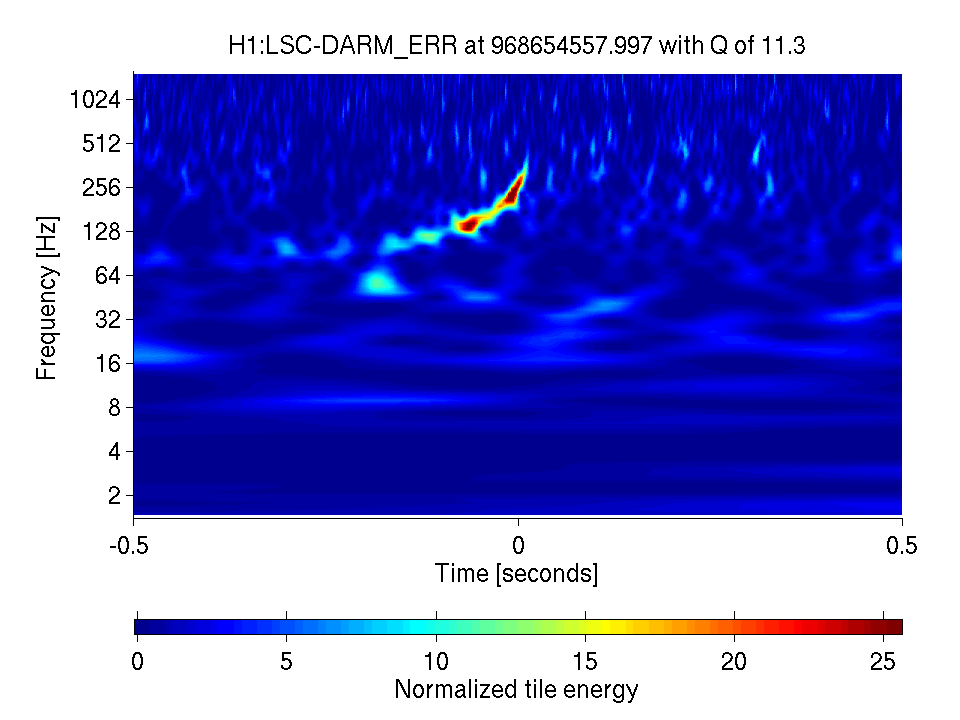
\includegraphics[width=0.5\linewidth]{figures/detchar/968654557_997314453_H1_LSC-DARM_ERR_1_00_spectrogram_whitened.png}
  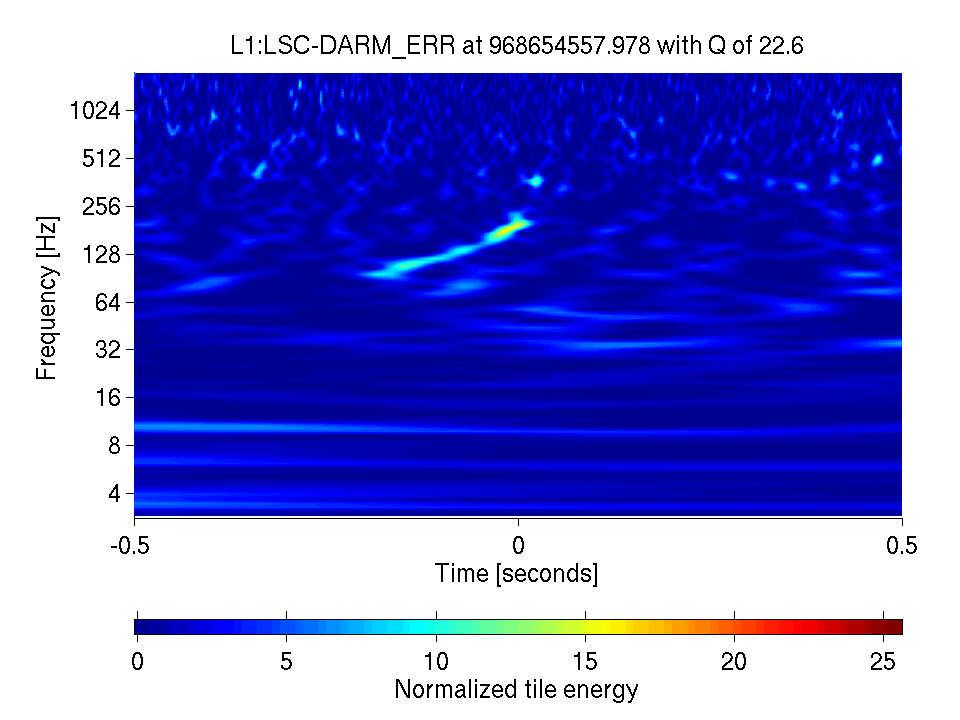
\includegraphics[width=0.5\linewidth]{figures/detchar/968654557_978027343_L1_LSC-DARM_ERR_1_00_spectrogram_whitened.png}
  \caption{H1 (left) and L1 (right) Omega scans of the injection as
generated by daily ihope.  Note the ``chirp'' shape which is the
expected pattern from a compact binary inspiral.}
  \label{f:daily_ihope_dog_omega}
\end{figure}%

\subsection{False Alarm Rate Estimate}

% https://www.lsc-group.phys.uwm.edu/ligovirgo/cbcnote/DailyDogHistograms

In order to determine the significance of this candidate event it was
necessary to compare it against the background.  The first such
comparison ranked the event against background triggers from the
two-week analysis in which it occurred as part of the standard ihope
pipeline.  However, the event had a larger combined new SNR value than
all background triggers, and hence had a false alarm probability of
zero.

In order to provide a more meaningful bound it was necessary to
increase the analysis time and/or number of slides to probe the
background more deeply. This is a complex and time-consuming process,
see (s6 paper) for details.  While this was underway we could begin to
bound the significance from daily ihope results.  This was done by
plotting histograms of all triggers throughout S6 and locating the
candidate triggers in the resulting distribution.  This analysis
differs from the full ihope pipeline in several respects.  However,
the goal was not a publishable result but only a rapid estimate.

To parallel the full analysis the results were broken into mass bins.
The low mass bin spans chirp masses up to $3.48\msun$, the medium mass
bin from $3.48-7.40 \msun$.  Likewise, category 1,2 and 3 vetoes were
applied to parallel the results of the full search.  30-millisecond
clustering was chosen to parallel the clustering used in the full
search.  There are several ways of reporting the new SNR of the
injection; the largest values reported by daily ihope, the largest
single-detector values reported by the full search, and the component
values of the largest combined new SNR reported by the full search.
All of these options are included on the plot.


The results are shown in figure \ref{f:daily_histogram_low} for the
low-mass bin and \ref{f:daily_histogram_medium} for the medium-mass
bin.  The result in both bins is qualitatively the same.  The
injection is close to the loudest event in H1 for all measures of new
SNR.  The injection does not stand out as far in L1, which was known
to be glitchier over the course of S6.


\begin{figure}
  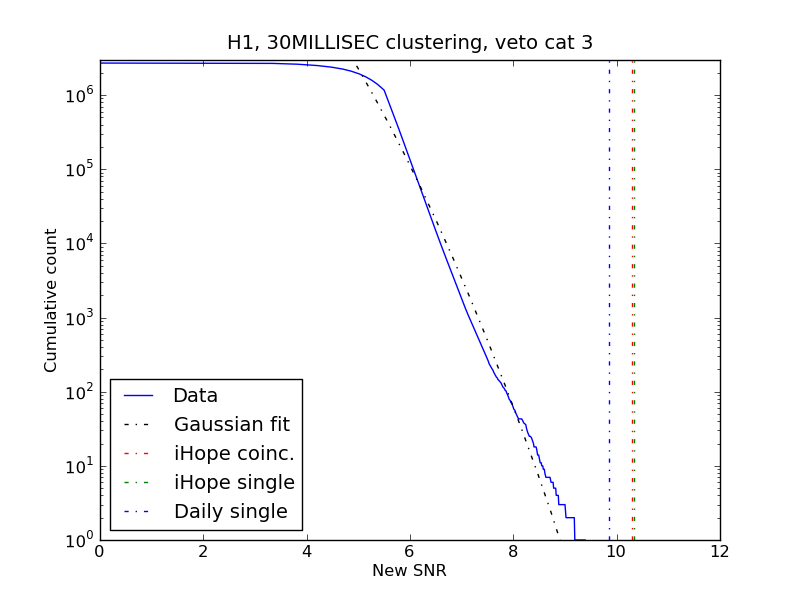
\includegraphics[width=0.5\linewidth]{figures/detchar/LM_H1_30MILLISEC_3_hist.png}
  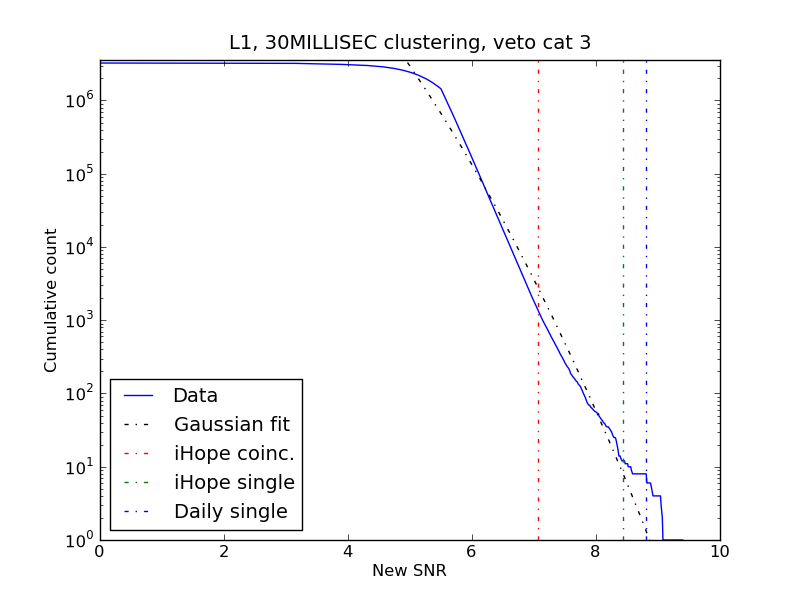
\includegraphics[width=0.5\linewidth]{figures/detchar/LM_L1_30MILLISEC_3_hist.png}
  \caption{Significance of the blind injection in the low-mass bin in 
H1 (left) and L1 (right).  Note the cumulative counts levels off
around between 5 and 5.5, indicating that there are few triggers with
smaller values.}
  \label{f:daily_histogram_low}
\end{figure}%



\begin{figure}
  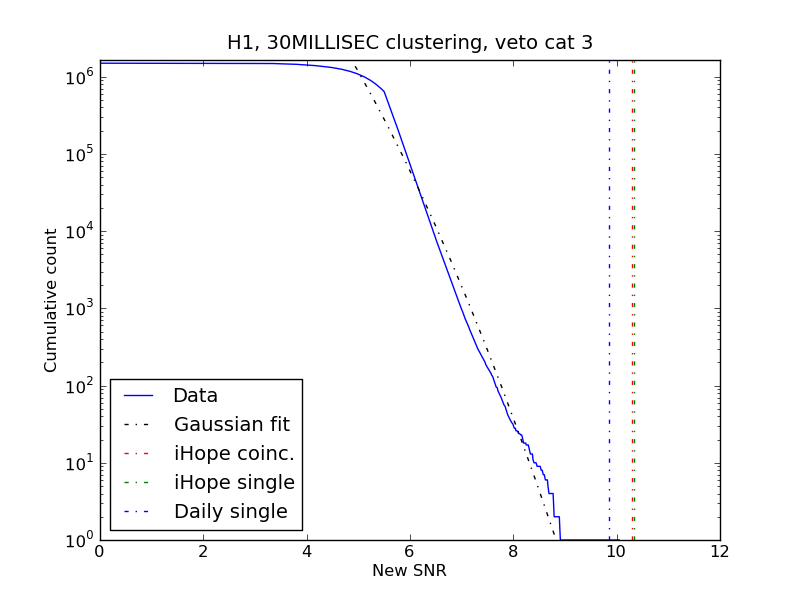
\includegraphics[width=0.5\linewidth]{figures/detchar/MM_H1_30MILLISEC_3_hist.png}
  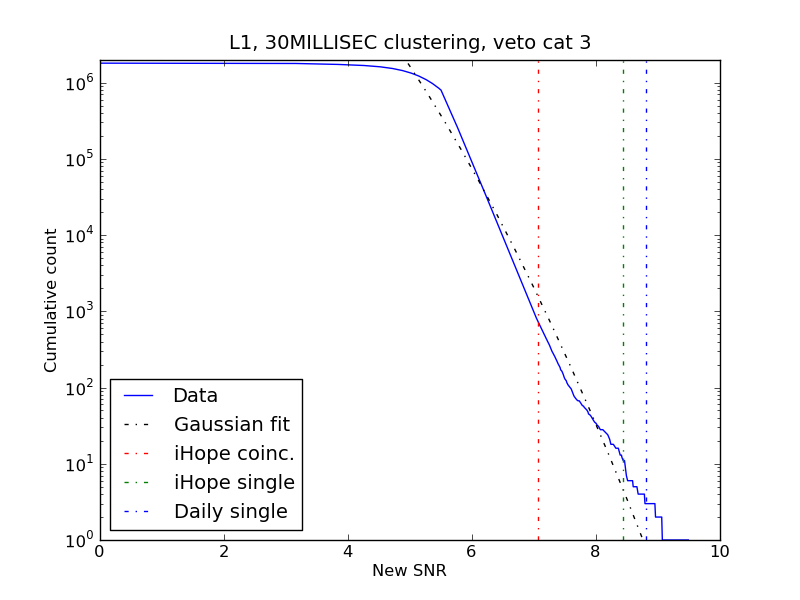
\includegraphics[width=0.5\linewidth]{figures/detchar/MM_L1_30MILLISEC_3_hist.png}
  \caption{Significance of the blind injection in the medium-mass bin in 
H1 (left) and L1 (right).  Note the cumulative counts levels off
around between 5 and 5.5, indicating that there are few triggers with
smaller values.}
  \label{f:daily_histogram_medium}
\end{figure}%


From these results we can attempt to estimate a false alarm rate for
the injection as follows.   Model coincident triggers as a Bernoulli
trial where ``success'' is obtaining a coincidence with combined new
SNR greater than or equal to that of the injection.  Denote the
probability of success in a single trial as $P$.  Then the probability
of obtaining the first success after $k$ trials is a geometric
distribution, $Prob(k) = P(1-P)^{k-1}$, and the expected number of
trials before success is $1/P$.  Dividing this by the estimated number
of coincident triggers in a year gives the estimated number of years
required to obtain such a trigger by chance.

The rate of coincident triggers, $R$, in the full search was estimated
by choosing a few analysis chunks and dividing the number of H1L1
triggers by the analysis time, both of which are reported after the
coincidence step.  The average rate is approximately 0.004
coincidences per second of analysis time, or $N=126,144$ per year.
This is combined across all mass bins, the result will therefore be an
upper limit for any particular bin.

% CIT:
% /archive/home/sprivite/S6/lowmass/s6d_weeks33_34/968803143-970012887/full_data
% for i in `/bin/ls | grep H1L1-COIRE_FIRST_FULL_DATA `
% do
%  grep 'amount of time analysed' $i | cut -f7 -d' '
% done | awk '{s+=$1} END {print s}'
% 135254
%
% for i in `/bin/ls | grep H1L1-COIRE_FIRST_FULL_DATA `
% do
%  grep 'reconstructed' $i | cut -f7 -d' '
% done | awk '{s+=$1} END {print s}'
%
% 523
% so 523 / 135254 = 0.00387 coinc/sec
%
%
% LHO (dog)
% /archive/home/mtwest/CBC-s6d/weeks_31-32/lowmass_run/967593543-968803287/full_data
% Gives 
% 886 / 244515 = 0.00362 coinc/sec


We estimate $P$ by assuming a probability density function in each
detector of the form

\begin{equation}
P(\rho_\textrm{new}) = \left\{
  \begin{array}{lr}
    0  & \rho < 5.5 \\
    \exp\left(-\frac{\rho^2}{2\sigma^2}\right) & \rho_\textrm{new} \geq 5.5 \\
  \end{array} \right.
\end{equation}

The lower cutoff is approximate.  We do not threshold on new SNR, and
while we do threshold on$\rho > 5.5$ it is possible for $\chisq$ to
push the resulting new SNR down.  In addition, due to clustering, the
probability of obtaining low new SNR triggers is suppressed.  The fit
to the Gaussian portion of the curves is show on  figures
\ref{f:daily_histogram_low} and \ref{f:daily_histogram_medium}, and
the obtained values are shown in table \ref{tab:daily_ihope_sigmas}.

\begin{table*}
\begin{center}
\begin{tabular}{l | l l}
   & $\sigma_H$ & $\sigma_L$ \\
\hline
Low mass bin    & 0.98 & 0.96 \\
Medium mass bin & 0.99 & 0.97 \\
\end{tabular}
\end{center}
  \caption{$\sigma$ values obtained by fitting Gaussians to daily
ihope trigger counts.}
  \label{tab:daily_ihope_sigmas}
\end{table*}

The joint PDF is then

\begin{equation}
P(\rho_H,\rho_L) = \frac{1}{A}
\int_{\rho_L = 5.5}^{\sqrt{\rho_i^2 - \rho_L^2}}
\int_{\rho_H = 5.5}^{\sqrt{\rho_i^2 - 5.5^2}}
\exp\left(-\frac{\rho_H^2}{2\sigma^2}\right)
\exp\left(-\frac{\rho_L^2}{2\sigma^2}\right)
\,d\rho_H
\,d\rho_L
\end{equation}

where $A$ is the normalization obtained by taking the upper limits of
both integrals to infinity.  This may be simplified by means of the
substitutions

\begin{align*}
s      &= \frac{\rho_H}{\sqrt{2}\sigma_H} \\
s_{\mathrm{low}}  &= \frac{5.5}{\sqrt{2}\sigma_H} \\
s_{\mathrm{high}} &= \frac{sqrt{\rho_i^2 - 5.5^2}}{\sqrt{2}\sigma_H} \\
t      &= \frac{\rho_L}{\sqrt{2}\sigma_L} \\
t_{\mathrm{low}}  &= \frac{5.5}{\sqrt{2}\sigma_L} \\
t_{\mathrm{high}}(s) &= \frac{\sqrt{\rho_i^2 - 2 \sigma_H^2 s^2}}{\sqrt{2}\sigma_L} \\
\end{align*}

in terms of which the normalization is

\begin{equation}
A = \frac{\pi}{2} \sigma_x \sigma_y \left[
1 - \erf(s_{\mathrm{low}}) - \erf(t_{\mathrm{low}}) + \erf(s_{\mathrm{low}})\erf(t_{\mathrm{low}})
\right]
\end{equation}

where $\erf$ is the error function.  The probability of obtaining a
trigger with combined new SNR larger then the injection is then

\begin{align*}
P &= 1 - \frac{\pi\sigma_L \sigma_H}{2 A} \bigg[
\frac{2}{\pi} \int_{s_{\mathrm{low}}}^{s_{\mathrm{high}}} e^{-s^2}
\erf(t_{\mathrm{high}}(s))\,ds \nonumber \\
&\quad - \erf(t_{\mathrm{low}}) \erf(s_{\mathrm{high}})  
+ \erf(s_{\mathrm{low}}) \erf (t_{\mathrm{low}}) \bigg] \\
\end{align*}


\iffalse
\begin{equation}
P(\rho_H,\rho_L) = 
\frac{4}{2\pi \sigma_H \sigma_L} 
\exp\left(
-\frac{\rho_H^2}{2\sigma_H^2} -\frac{\rho_L^2}{2\sigma_L^2}
\right)
\end{equation}

where the factor $4$ comes from considering only the quadrant where
both SNRs are positive.

The probability of obtaining a trigger with new SNR greater than
that of the injection, $\rho_i$, is then

\begin{align}
P = 
\frac{4}{2\pi \sigma_H \sigma_L} 
\int_{\rho_H^2 + \rho_L^2 > \rho_i^2}
\exp\left(
-\frac{\rho_H^2}{2\sigma_H^2} -\frac{\rho_L^2}{2\sigma_L^2}
\right)
\,d\rho_H\,d\rho_L
\end{equation}

Introducing a temporary variable $M = \rho_L \sigma_H/\sigma_L$, going to polar
coordinates, evaluating the integral over $r$ and simplifying gives


\begin{equation}
P(\rho_c^2 > \rho_i^2|\textrm{coincidence}) = 
\frac{1}{2\pi \sigma_H \sigma_L} 
\frac{\sigma_L}{\sigma_H}
\int_{\rho_H^2 + (\sigma_L/\sigma_H)^2 M^2 \leq \rho_i^2}
\exp\left(
-\frac{\rho_H^2}{2\sigma_H^2} -\frac{M^2}{2\sigma_H^2}
\right)
\,d\rho_H\,dM
\end{equation}



\begin{equation}
P = 
\frac{1}{2\pi \sigma_H \sigma_L} 
\frac{\sigma_L}{\sigma_H}
\int_{r^2\cos^2\theta + (\sigma_L/\sigma_H)^2 r^2\sin^2\theta \leq \rho_i^2}
\exp\left(
-\frac{r^2\cos^2\theta}{2\sigma_H^2} -\frac{r^2\sin^2\theta}{2\sigma_H^2}
\right)
r\, dr\, d\theta
\end{equation}


\begin{equation}
P = 
\frac{1}{2\pi \sigma_H \sigma_L} 
\frac{\sigma_L}{\sigma_H}
\int_{r^2\cos^2\theta + (\sigma_L/\sigma_H)^2 r^2\sin^2\theta \leq \rho_i^2}
\exp\left( -\frac{r^2}{2\sigma_H^2} \right)
r\, dr\, d\theta
\end{equation}


\begin{equation}
P = 
\frac{1}{2\pi \sigma_H \sigma_L} 
\frac{\sigma_L}{\sigma_H}
\sigma_H^2
\int_0^{2\pi}
\left( 1 - 
\exp\left(
  -\frac{1}{2\sigma_H^2} 
   \frac{\rho_i^2}
        {\cos^2\theta + (\sigma_L/\sigma_H)^2 \sin^2\theta} 
\right)
\right)
d\theta
\end{equation}

\begin{equation}
P = \frac{4}{2\pi}
\int_0^{\pi/2}
\exp\left(
  -\frac{1}{2} 
   \frac{\rho_i^2}
        {\sigma_H^2 \cos^2\theta + \sigma_L^2 \sin^2\theta} 
\right)
d\theta
\end{equation}

\fi

This integral can be evaluated numerically.  Henceforth we focus on
the medium mass bin, as that was the bin with the most significant
trigger with a combined new SNR $\rho_i = 12.5$.  The result is
$P = 1.4 \times 10^{-20}$, which gives a false alarm rate of
1 event in 

\begin{equation}
\frac{1.0}{1.4 \times 10^{-26}} \times \frac{1}{126,144}
= 8.6\times 10^{24}\quad\textrm{years}
\end{equation}

This grossly underestimates the FAR calculated using time slides based
on the full analysis, which gives 1 in 7,000 years.  There is no
simple factor that explains this discrepancy; the two analyses are
significantly different, and in particular the real search uses a
two-stage pipeline that makes it difficult to reason about the results
based on the output of single-stage single-ifo triggers.  However,
this does suggest an alternative method to estimate FARs for a
single-stage pipeline which is currently in development.

\subsection{Front-end code verification}

% http://www.gravity.phy.syr.edu/dokuwiki/doku.php?id=larne:frontendcode
% https://dcc.ligo.org/cgi-bin/private/DocDB/ShowDocument?docid=39122
% https://dcc.ligo.org/cgi-bin/private/DocDB/ListBy?authorid=272

Before the collaboration could claim a detection it was necessary to
perform extensive checks to remove, or at least reduce, the
possibility that the trigger was due to any source other than a
gravitational wave.  Consequently many components of the
interferometer were subject to scrutiny.  One such component was the
\emph{front-end control code}, which is responsible for \checkme{FILL
IN DETAILS}.  This code is updated occasionally as new systems are
added or bugs are found and fixed.   To verify that the most recent
change preceding the event did not significantly change the behavior
of the instruments we compared histograms of triggers from daily ihope
before and after these changes.

Two weeks prior to and following the most recent code changes at each
site were selected.  SNR histograms are shown in figure \ref{f:code_changes}.
There is a slight variation in H1, somewhat larger in L1.  More
rigorous testing could have been done, one possibility would be to
determine rates from several two-week periods before the code change
in order to estimate the standard deviation in each SNR bin, and then
checking whether the rates after the change fall within one sigma.
However, the detection committee did not feel this level of analysis
was necessary, and based on the plots in figure \ref{f:code_changes}
concluded:


\begin{figure}
  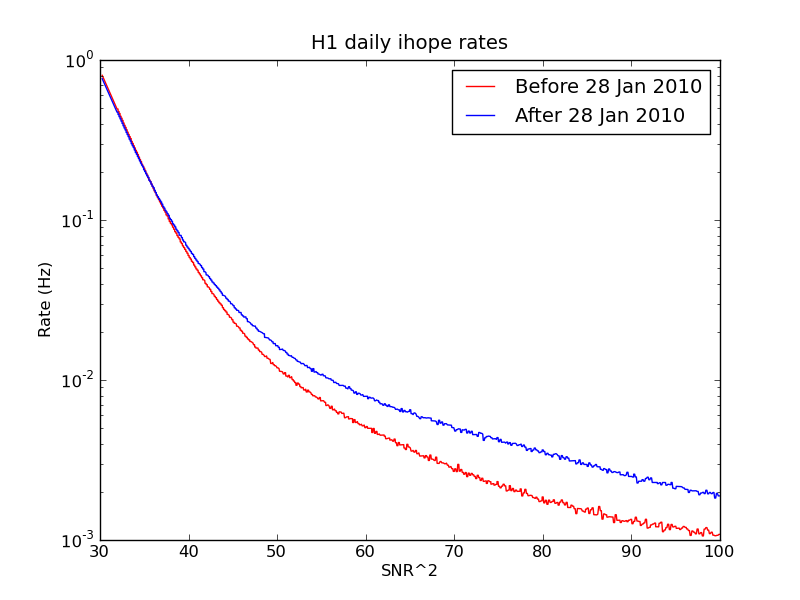
\includegraphics[width=0.5\linewidth]{figures/detchar/frontendtest_h1_log_2.png}
  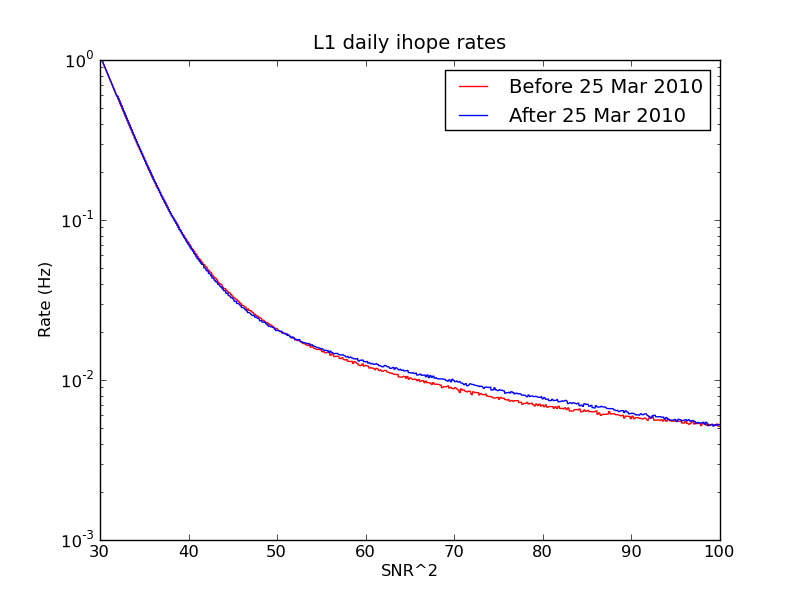
\includegraphics[width=0.5\linewidth]{figures/detchar/frontendtest_l1_log_2.png}
  \caption{SNR histograms comparing periods before and after 
front-end code changes at H1 (left) and L1 (right).}
  \label{f:code_changes}
\end{figure}%


\begin{quote}
  Thus, to the extent allowed by the methods we adopted, there is no
  evidence for any malfunction in the front-end code of the
  interferometers. (cite https://dcc.ligo.org/cgi-bin/private/DocDB/ShowDocument?docid=39122)
\end{quote}

\subsection{Loud-SNR veto}

Through the S6 run the \emph{horizon distance}, the distance at which
the coalesence of an optimally-oriented binary system consisting of
two $1.4 \msun$ neutron stars would have an SNR of 8, was roughly 30
Mpc.  The SNR scales inversely with distance, hence the distance at
which we would expect to see such a system at, say, SNR 250 is 0.12
Mpc.  Assuming uniform volume distribution, this makes an SNR 250
event $6.4 \times 10^{-8}$ times less likely than an SNR 8 event.  
However, such loud glitches do occur in the data fairly often,
especially at L1 due to a glitch mechanism with a characteristic shape
but unknown cause.

Such loud glitches tend to have high $\chisq$ values which suppress
them.  However, around SNR 250 glitches tend to be accompanied by
additional triggers spanning $\pm 8$ seconds resulting from the
interaction of the filter with the inverse spectrum truncation, see
section \ref{sec:ihope_data_conditioning}.  Some of these auxiliary
triggers can, by chance, have low $\chisq$ values and hence high new
SNR values, and can potentially interfere with the search.  This
suggests a CAT 4 veto centered on times of triggers with SNRs
exceeding 250 with 8 seconds of padding in both directions.  Such a
flag must be in place before the full run, making daily ihope the
obvious choice for generating the flags.

This scheme was implemented starting on June 26, 2010, coinciding with
the portion of the run designated S6D.  An example of its
effectiveness is shown in table \ref{tab:daily_ihope_loud_flag} which
shows the efficiency and deadtime off the flag applied to triggers
from the full analysis after CAT 1, for the two weeks containing the
blind injection.  The efficiency to deadtime ratio is greater than 1,
although still relatively small.  Still, the flag was deemed useful as
it removed triggers we could not have easily claimed were due to a
gravitational wave.

\begin{table*}
\begin{center}
\begin{tabular}{lrrcrrcc}
\hline
ifo & Triggers & Vetoed & Efficiency & Time
& Vetoed & Dead-  & Ratio \\
 & (Count) & (Count) &  & (sec) & (sec) & time (sec) &  \\
\hline
L1  & 2890507 & 12578 & 0.43 & 798720 & 880 & 0.11 & 3.95 \\
H1  & 1692904 &  6452 & 0.38 & 647168 & 416 & 0.06 & 5.92 \\
\end{tabular}
  \caption{Effectiveness of the ``SNR $>$ 250'' flag over the weeks
09/04/2010  to 09/17/2010.  Note that the flag was used almost twice
as often in L1 as H1, although there is only 23\% more analysis time.
This is another indication that L1 was glitchier overall.}
  \label{tab:daily_ihope_loud_flag}
\end{center}
\end{table*}

% tot_time, tot_count
% veto_time, veto_count

% $ ./check_flags.py L1
% 798720 2890507
%    880   12578
% $ ./check_flags.py H1
% 647168 1692904
%    416    6452


